%%%%%%%%%%%%%%%%%%%%%%%%%%%%%%%%%%%%%%%%%%%%%%%%%%%%%%%%%%%%%%%%%%%%%%%%%%%%%
%%%                             Description                               %%%
%%%%%%%%%%%%%%%%%%%%%%%%%%%%%%%%%%%%%%%%%%%%%%%%%%%%%%%%%%%%%%%%%%%%%%%%%%%%%
\newpage
\subsection{DESCRIPTION}
\label{sec:description}
The application title following the \DESCRIPTION{}
may be given as string or single word with no
spaces. It will be displayed as title string in all windows of that
application.

Each of the \INTENS{} objects has its own description block. All blocks
(except \verb+language_description+) can be repeated in any sequence
as long as the referenced identifiers within one block are declared in one of the
previous blocks.

Description blocks \DATAPOOL{} and \UIMANAGER{} are \underline{mandatory}.

\index{DESCRIPTION@\DESCRIPTION!application title}
\index{DESCRIPTION@\DESCRIPTION!description blocks}
\index{END@\END .!end of description file}
\input{diagrams/description}
\input{diagrams/descriptions}

\begin{tabularx}{\textwidth}{l|X}
description block & description \\
\hline
IDENTIFIER / string & application title (see above). \\
\HELPFILE         & section \nameref{sec:helpfile} page \pageref{sec:helpfile}. \\
\DATAPOOL         & section \nameref{sec:datapool} page \pageref{sec:datapool}. This block is {\bfseries mandatory}. \\
\STREAMER         & section \nameref{sec:streamer} page \pageref{sec:streamer}. \\
\UIMANAGER        & section \nameref{sec:uimanager} page \pageref{sec:uimanager}. This block is {\bfseries mandatory}. \\
\OPERATOR         & section \nameref{sec:operator} page \pageref{sec:operator}. \\
\FUNCTIONS        & section \nameref{sec:functions} page \pageref{sec:functions}. \\
\end{tabularx}

%%%%%%%%%%%%%%%%%%%%%%%%%%%%%%%%%%%%%%%%%%%%%%%%%%%%%%%%%%%%%%%%%%%%%%%%%%%%%
%%%                              Examples                                 %%%
%%%%%%%%%%%%%%%%%%%%%%%%%%%%%%%%%%%%%%%%%%%%%%%%%%%%%%%%%%%%%%%%%%%%%%%%%%%%%
\label{sec:descriptionexamples}

The following example shows a minimal configuration to give a first
practical view of \INTENS{}:


\begin{boxedminipage}[t]{\linewidth}
\begin{alltt}
// SEMAFOR Informatik & Energie AG
// Basel, Switzerland
//

\DESCRIPTION "Minimal Example";
\DATAPOOL
  \REAL\{\EDITABLE\} speed;
\END \DATAPOOL;

\UIMANAGER
   \FIELDGROUP
      g1( "speed:" speed "km/h" );
   \FORM
      f1\{\MAIN\}( (g1) );
\END \UIMANAGER;
\END.
\end{alltt}
\end{boxedminipage}

\vspace{0.5cm}

After reading the above configuration data
\INTENS{} has created a main window containing two text windows and
a fieldgroup as shown in figure below.
You will later see (section \nameref{sec:uimanager} on page
\pageref{sec:uimanager}) how to configure additional forms and how to
move the text windows to another form. \\
\vspace{0.5cm}

%%--------------minimal example-----------------------------------
\begin{figure}[h]\label{fig:minimalExample}
  \begin{center}
    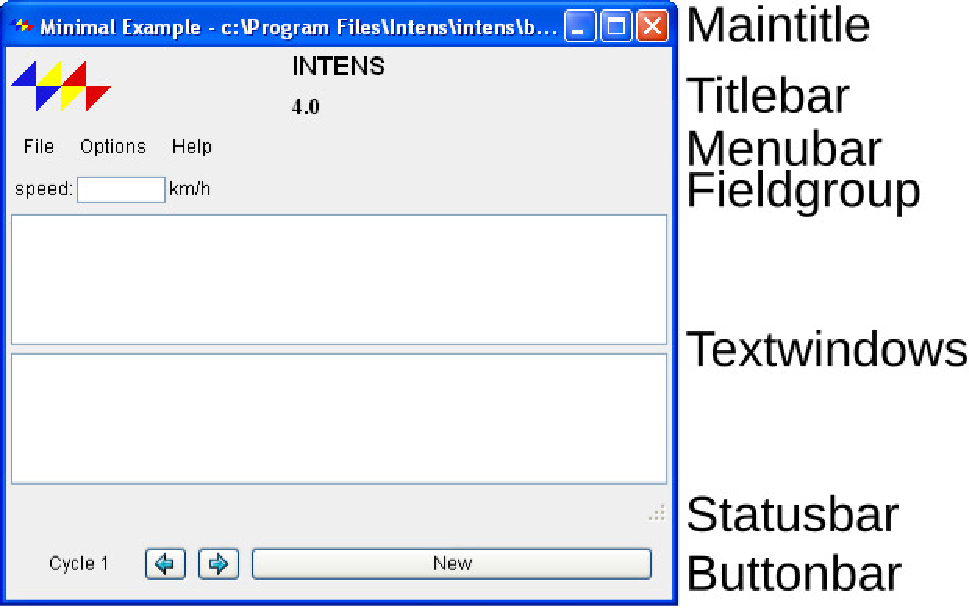
\includegraphics[width=0.6\linewidth]{grab_minimal}
  \end{center}
  \caption{Minimal example}
\end{figure}
\index{Maintitle!Minimal example}
\index{Titlebar!Minimal example}
\index{Menubar!Minimal example}
\index{FIELDGROUP@\FIELDGROUP!Minimal example}
\index{TEXT\_WINDOW@\TEXTWINDOW!Minimal example}
\index{Statusbar!Minimal example}
\index{Buttonbar!Minimal example}
